\documentclass[letterpaper]{article}
\usepackage{amssymb}
\usepackage{amsfonts}
\usepackage{amsmath}
\usepackage{stmaryrd}
\usepackage{graphicx}
\usepackage{subfigure}
\usepackage{pslatex}   % Good fonts psType 1 or \usepackage{mathptmx}
\usepackage{varioref}  % smart page, figure, table, and equation referencing
\usepackage{algorithm}
\usepackage{algorithmic}
%\usepackage{algorithm2e}
\usepackage{cancel}
\usepackage[small]{caption}
\usepackage{cancel}
\usepackage{tikz} 
\usepackage{pgf}
%\usepackage{fancy headings}

  \newcommand{\eqnref}[1]{Eq. (\ref{#1})}                % Eq. (no)
  \newcommand{\figref}[1]{Figure \ref{#1}}                % Figure (no)
  \newcommand{\tblref}[1]{Table \ref{#1}}                % Table (no)
  \newcommand{\secref}[1]{Section \ref{#1}}                % Section (no)
  \newcommand{\incfig}{\centering\includegraphics*}  % Centered 
  \newcommand{\comment}[1]{\COMMENT{ \textcolor{blue}{ #1} }  }

%DG integrals
\newcommand{\pd}[2]{\frac{ \partial #1}{\partial #2}}
\newcommand{\volint}[1]{ \sum_{e \in \mathcal{T}_{h}}\int_{\Omega_k} #1 d\Omega_{e} }  
\newcommand{\surfint}[1]{\sum_{i\in \mathcal{I}_{h}}\int_{\Gamma^{i}} #1 ds}
\newcommand{\bsurfint}[1]{\sum_{b\in \mathcal{B}_{h}}\int_{\Gamma^{b}} #1 ds}
% Operators
\newcommand{\frechd}[2]{ #1'_{\left[ #2 \right]} }%\left( #3\right)} 
\newcommand{\diver}[1]{\nabla \cdot #1}
\newcommand{\abs}[1]{\left \lvert #1 \right \rvert}
\newcommand{\avg}[1]{\left\{ #1 \right\} }
\newcommand{\jump}[1]{\llbracket #1 \rrbracket}
\newcommand{\mat}[1]{\left[ #1 \right]}
\newcommand{\paren}[1]{\left( #1 \right)}
\newcommand{\sparen}[1]{\left[ #1 \right]}
\newcommand{\twonorm}[1]{\parallel #1 \parallel_{2}}
%variables
\newcommand{\hb}[1]{ {\bf #1}_{h} } % \hb for discrete symbol _{h} and bolded for vector in fields
% Fluxes 
\newcommand{\fc}{\vec{{\bf F}}_{c} \paren{\hb{u}}   }
\newcommand{\fv}{\vec{{\bf F}}_{v} \paren{\hb{u},\nabla \hb{u}} }
\newcommand{\fav}{\vec{{\bf F}}_{ad} \paren{ \epsilon,\hb{u},\nabla \hb{u} } }
\newcommand{\ec}{\vec{{\bf E}}_{c} \paren{\hb{u}}   }
\newcommand{\ev}{\vec{{\bf E}}_{v} \paren{\hb{u},\nabla \hb{u}} }
\newcommand{\eav}{\vec{{\bf E}}_{ad} \paren{ \epsilon,\hb{u},\nabla \hb{u} } }

\newcommand{\hc}{\mathcal{H}_{c} \paren{ \hb{u}^{+},\hb{u}^{-},\vec{n} } }  
\newcommand{\hv}{\mathcal{H}_{v} \paren{ \hb{u},\hb{u}^{-},\phi_{i}^{+}, \phi_{i}^{-},\nabla \hb{u}^{+},\nabla \hb{u}^{-},
\vec{n} } }
\newcommand{\hav}{\mathcal{H}_{ad}\paren{ \epsilon^{+},\epsilon^{-},\hb{u}^{+},\hb{w}^{+}, \hb{w}^{-},\hb{u}^{-},\nabla \hb{u}^{+},\nabla \hb{u}^{-},\vec{n} } }
\newcommand{\hcb}{\mathcal{H}_{c}^{b} \paren{ \hb{u}^{b} \paren{ \hb{u}^{+} },\vec{n} } } 
\newcommand{\hvb}{\mathcal{H}_{v}^{b} \paren{ \hb{u}^{b} \paren{\hb{u}^{+}},\phi_{i}^{+},\nabla \hb{u}^{+},\vec{n} } }
\newcommand{\havb}{\mathcal{H}_{ad}^{b} \paren{ \epsilon^{+}, \hb{u}^{b}\paren{ \hb{u}^{+}},{\bf w}^{+}, \nabla \hb{u}^{+},\vec{n} } }
%Non-linear variables
\newcommand{\Resid}[1] {{\bf R}(#1)}
\newcommand{\Residp}[1] {{\bf R}_{p}(#1)}
%FIgures
\newcommand{\figwidth}{.48\textwidth}
\newcommand{\lfigwidth}{.68\textwidth} %small version .68, large version .75
%%% Footer
%\lfoot[\fancyplain{}{}]{Approved for public release \\ distribution unlimited.}
\newcommand{\createav}{CREATE\textsuperscript{TM}-AV }

\title{Boundary Mapping}
\author{Nicholas K. Burgess}
\begin{document}
\maketitle
\section{Introduction} 
Computing the residual contribution from domain boundaries requires the evalutation of surface integrals.  Computing these integrals requires quadrature surface entities of the mesh (lines in 2-D and faces in 3-D).  Employing a surface quadrature rule can be somewhat confusing since the quarature rule specifies points and weights on a surface which is one dimension smaller than the mesh entities.  For example if one is solving a PDE in 2-D then surface quadrature is specified by a set of points $\xi_{qp}=\left\{(s_{qp})\right\}$, where $s$ is a surface coordinate.  If one is solving a PDE in 3-D then surface quadrature is specified by a set of points $\vec{\xi}_{qp} ={(u_{qp},v_{qp})}$, where $u,v$ is a surface coordinate pair.    

\section{Evaluating Polynomials on Boundaries}
The surface quadrature points are specified in a different lower dimension set of coordinates than the element as a whole.  However, the basis functions are defined in the standard element and therefore require element and not face coordinates.  Essentially we require a map $X(s): \mathbb{R}^{1} \mapsto \mathbb{R}^{d}$ for mapping a 1-D entity to a d-D entity.  We also require a map $X(u,v) :\mathbb{R}^{2} \mapsto \mathbb{R}^{d}$, for mapping 2-D to d-D.    

\subsection{Example mapping from 1-D to 2-D}
Consider an edge on a triangle (depited in \figref{fig:tri}).  
\begin{figure}
\centering
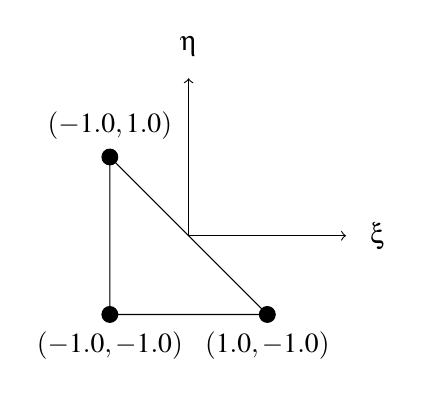
\begin{tikzpicture}
\draw[fill=black] (-1,-1) circle(.1cm) -- (1,-1) circle(.1cm) -- (-1,1) circle(.1cm) -- (-1,-1) circle(.1cm);
\draw (-1,-1.4)  node {$(-1.0,-1.0)$} (1,-1.4) node {$(1.0, -1.0)$} (-1,1.4) node {$(-1.0,1.0)$};
\draw[arrows=->] (0,0) -- (2,0);
\draw (2.4,0) node {$\xi$};
\draw[arrows=->] (0,0) -- (0,2);
\draw (0, 2.4) node {$\eta$};
\end{tikzpicture}
\caption{2-D Triangle element.}
\label{fig:tri}
\end{figure}

Now it's relatively trival to see what the coordinates are for any particular edge of the triangle.  However, given a coordinate $s\in[-1,1]$ in 1-D on an arbitrary line segment one can obtain any edge of the triangle.  All that one has to do is define $\xi(s)$ and $\eta(s)$ and since we are mapping a straight line segment to a straight triangular edge we can use linear functions to define these mappings.  In fact you should have guessed by now which functions you should use, which are $\phi_{1}=(1-s)/2$ and $\phi_{2}=(1+s)/2$.  The maps are defined as 
\begin{equation}
\begin{split}
\xi(s) = \frac{1-s}{2}\xi_{1} + \frac{1+s}{2}\xi_{2}
\eta(s) = \frac{1-s}{2}\eta_{1} + \frac{1+s}{2}\xi_{2}
\end{split}
\end{equation}

The following table shows the coefficients and final expression for mapping each edge of the triangle in \figref{fig:tri}. 

\begin{table}[h!]
\centering
\caption{Energy norm surface contribution of common external aerodynamics boundary conditions.}
\begin{tabular}{| c | c | c | c | c |}
\hline
Triangle Edge Number & $(\xi_{1},\eta_{1})$ & $(\xi_{2},\eta_{2})$ & $\xi(s)$ & $\eta(s)$ \\
1 & $(-1,-1)$ & $(1,-1)$ & $\xi(s) = s$ & $\eta(s) = -1$ \\
2 & $(1,-1)$  & $(-1, 1)$ & $\xi(s) = s$ & $\eta(s) = -s$ \\ 
3 & $(-1,1)$  & $(-1,-1)$ & $\xi(s) = -1$ & $\eta(s) = s$ \\ 
\hline
\end{tabular}\\
\label{tbl:}
\end{table}
This same techniques can be applied for faces and elements in 3-D and on any element where a linear basis can be defined.  The general proceedure is to formulate a nodal basis on the edge/face and then expand the $(\xi, \eta, \zeta)$ coordinates in a linear nodal basis on the edge/face.   

%%%%%%%%%%%%%%%%%%%%%%%%%%%%
\end{document}
